% GENI Lab_1.tex - GENI Lab 1 for Cloud Computing class (Spring 2015)
% Chanmann Lim - February 2015

\documentclass[a4paper]{article}

\usepackage[margin=1 in]{geometry}
\usepackage{listings}
\usepackage{graphicx}

\begin{document}
\title{CS 7001-03: Report for GENI Lab 1 - GENI Account Setup and Services Overview}
\author{Chanmann Lim\\ 
	\texttt{cl9p8@mail.mail.missouri.edu}}
\date{February 17, 2015}
\maketitle

% ---------------------------------------- 1 ----------------------------------------
\paragraph{1. } Screenshot of slice resource and Iperf results: \\
\begin{figure}[h!]
  \centering
    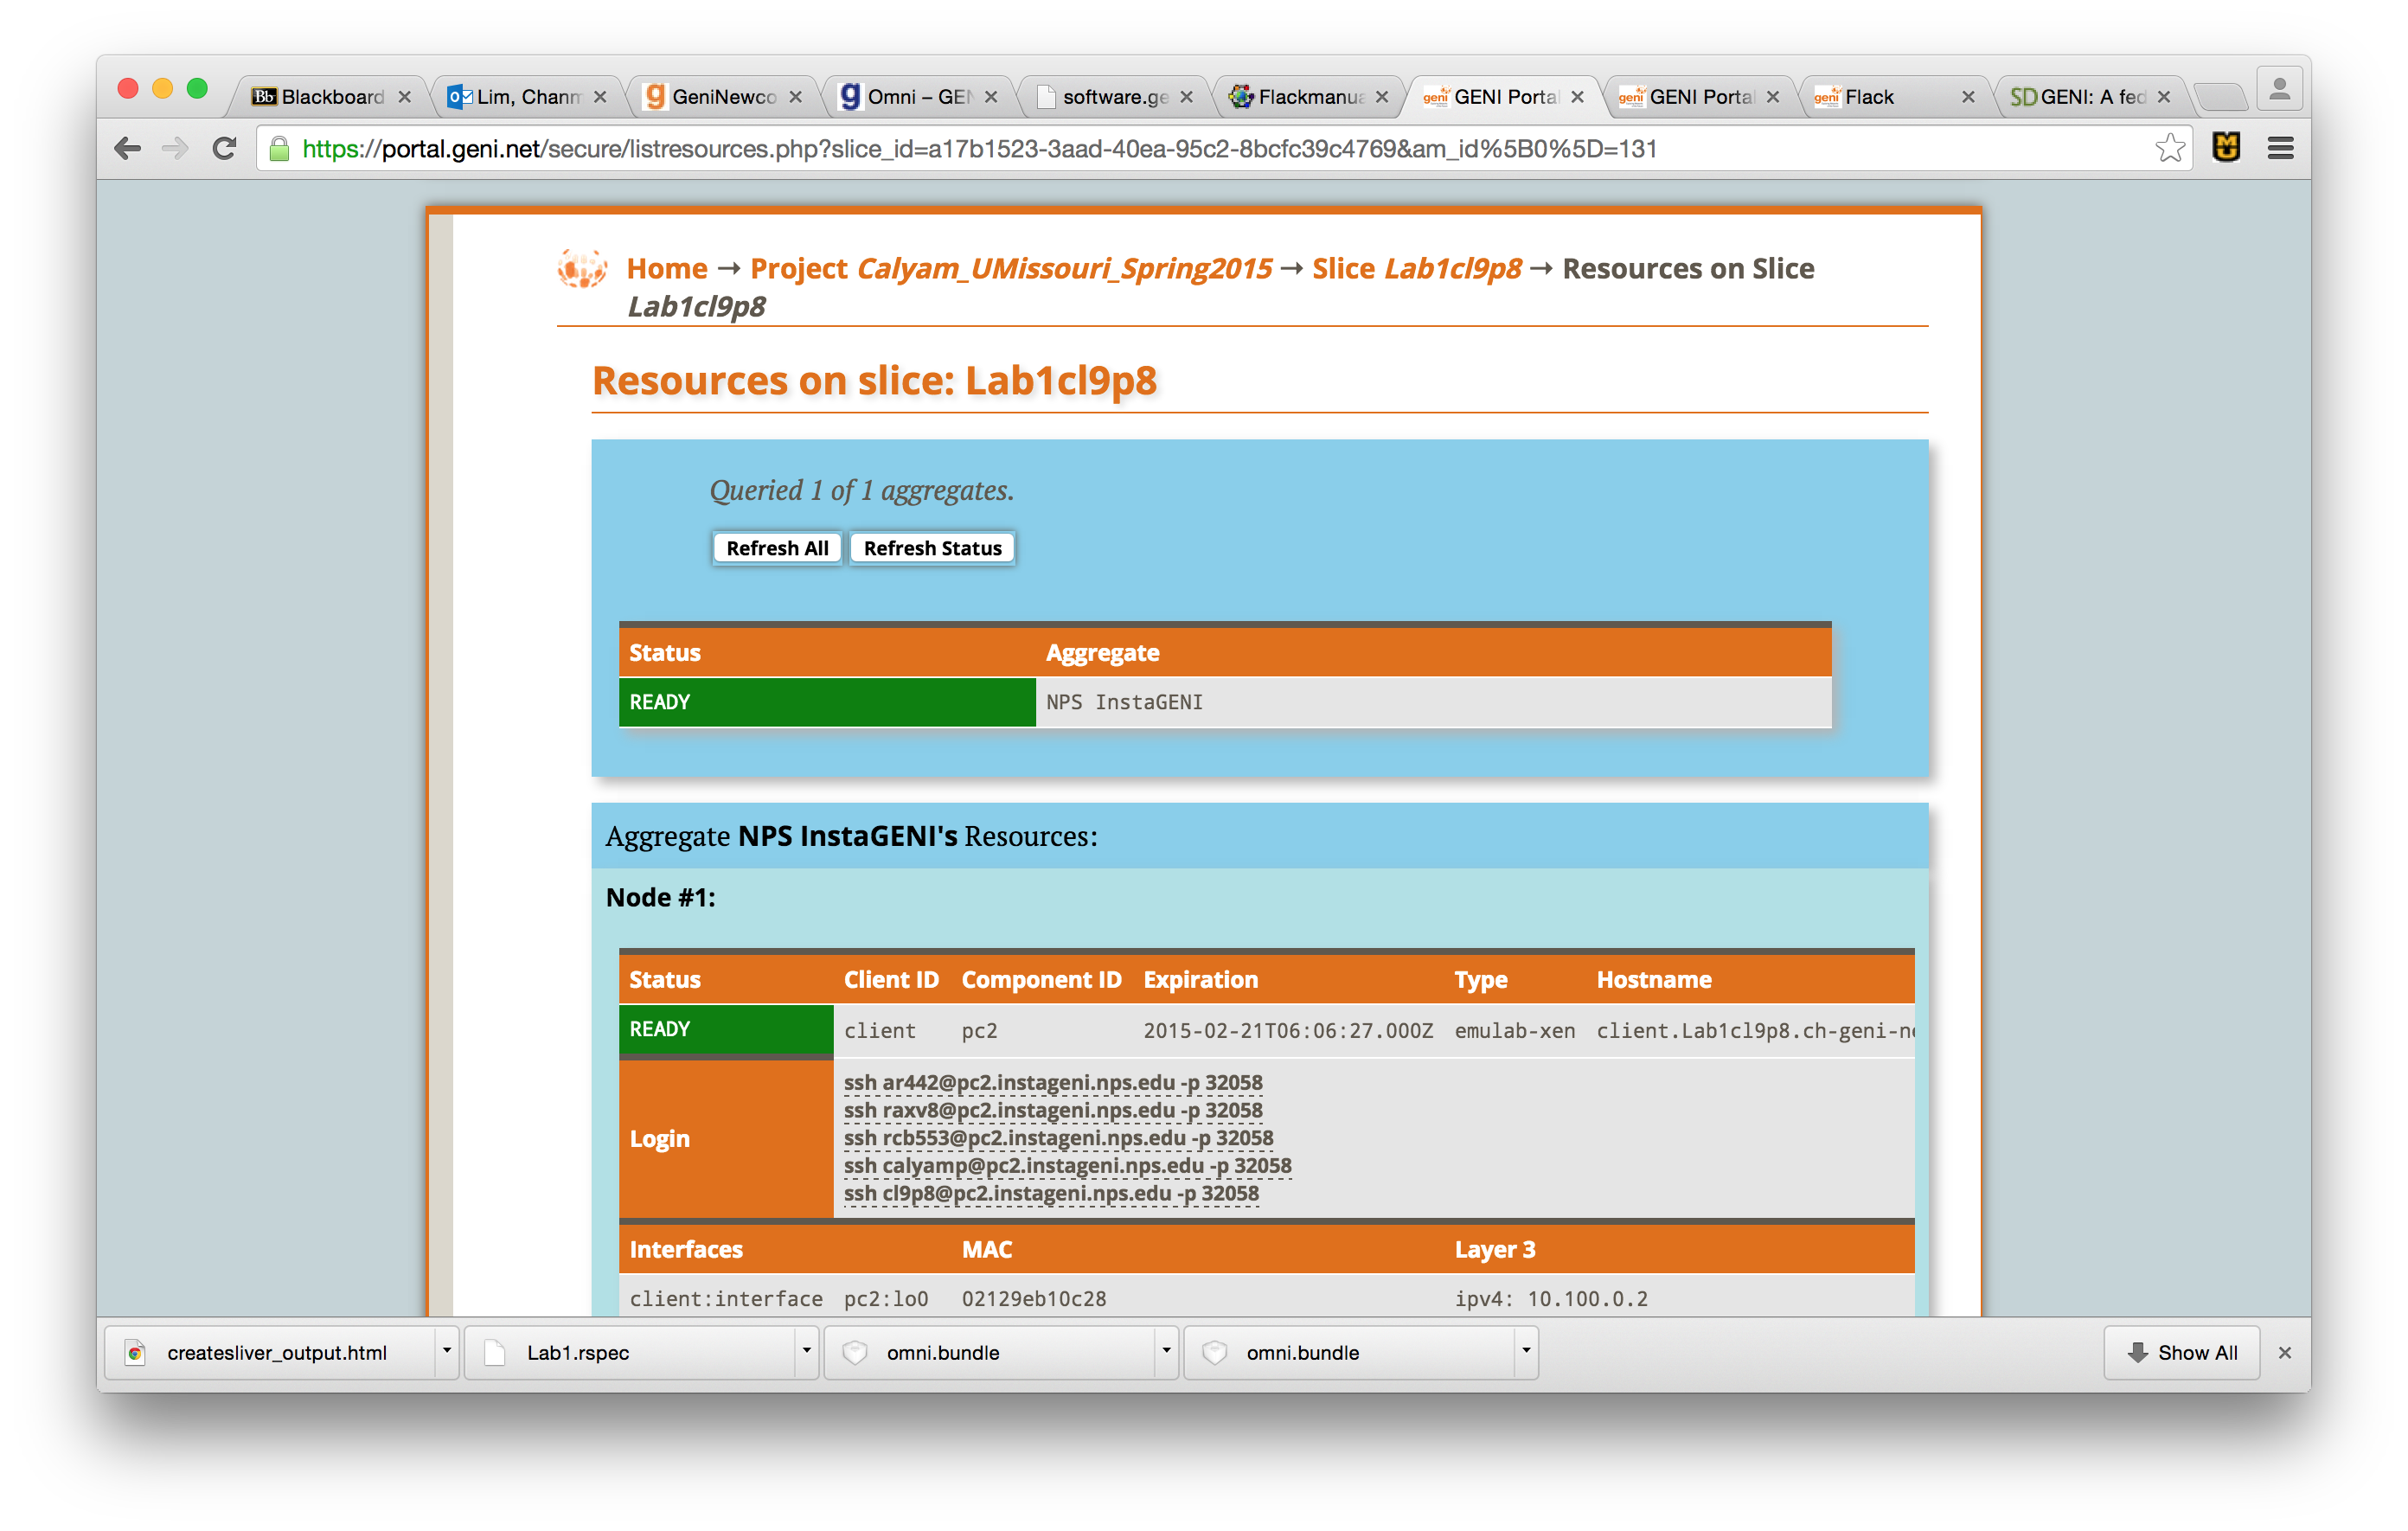
\includegraphics[scale=.32]{slice_resource.png}
  \caption{Slice resource}
\end{figure}

\begin{figure}[h!]
  \centering
    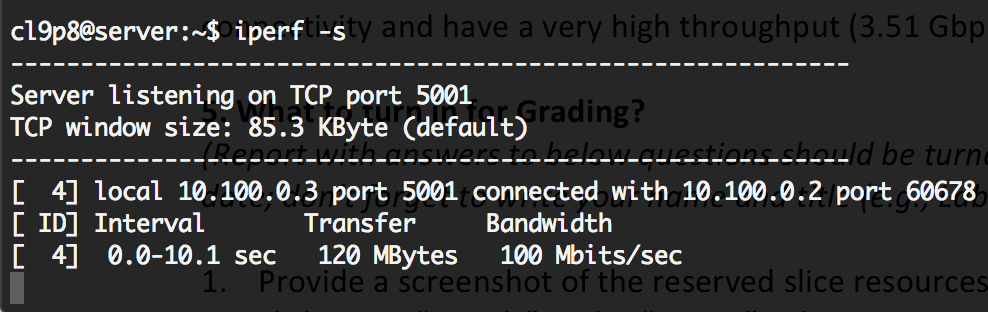
\includegraphics[scale=.5]{iperf_server.png}
  \caption{Iperf server}
\end{figure}

\begin{figure}[h!]
  \centering
    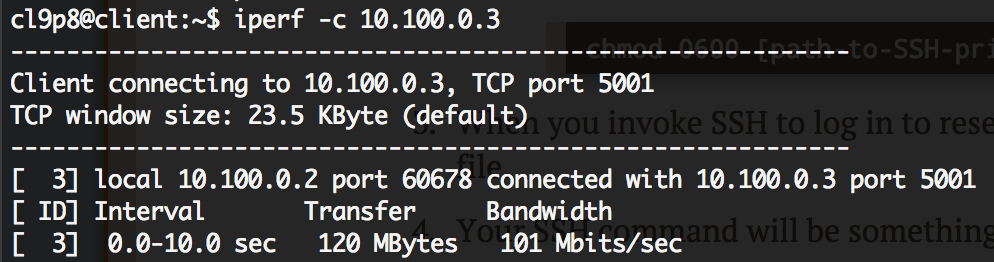
\includegraphics[scale=.5]{iperf_client.png}
  \caption{Iperf client}
\end{figure}
\vfill

% ---------------------------------------- 2 ----------------------------------------
\paragraph{2. } The added capacities and benefits in performing an experiment in GENI (Global Environment for Network Innovations) Internet infrastructure versus commercial Internet infrastructure are (1) Large-scale experiment infrastructure for computing virtual machines, bare-machines and network links and switches (2) Non-IP connectivity between two virtual machines using Layer 2 and Layer 3 connection (3) Deep programmability using software-defined network to do network programming (4) Reproducibility to offer repeatable testing environment such as CPU and networking resource (5) Instrumentation and measurement tools for system analyses and controls.

\paragraph{3. } GENI terminologies:
\begin{description}
\leftskip 0.4in
\parindent -0.4in
	\item[Slice: ] \hfill \\is a shared testbed containing a network of virtualised resources (computing or network) to perform an experiment.
	\item[Sliver: ] \hfill \\is the resources (virtual or bare-metal) to be added to slices and different aggregates(capacities made available by resource providers) provide different types of sliver (compute, storage or network).
	\item[Aggregate manager: ] \hfill \\is the controller of a collection of aggregates to handle resources discovery and reservation.
	\item[Rspec: ] \hfill \\is the resource specification in the form of XML document used to communicate with aggregate manager.
\end{description}

\paragraph{4. } Then GENI portal provides Federated Identity and Access Management to allow MU students to use their Pawprint and password to login by registering its service under The Research \& Scholarship Category federation so that Identity Provider like MU will be in charge of verifying user identity then share a set of low-risk attributes back to GENI portal(the service provider).\\

The benefit of this approach is that (1) researchers can have access to the service provider sites without delay and the involvement from local identity provider(research institution) administrator, (2) it simplifies the regulatory policy and operational practices of the collaboration between Identity providers and the service providers, (3) it will broaden the global Research and Engineering community efforts.

\paragraph{5. } The role of "Experiment Control Tools" such as Omni, jFed and Flack in GENI are the facilitations of resources discovery and configuration in the pool of aggregate managers.\\

The advantage of using Omni command line tool over using the Flack GUI is the support for automating the resources reservation tasks using script.

\paragraph{6. } SSH keys are the identity information used during secure remote login session to get into the computing resource and SSL keys are the user's identity used during the communication session to aggregate manager API through secure sockets layer (SSL) such as HTTPS. 

\end{document}